\documentclass[12pt]{article}
\usepackage{hyperref}
\usepackage{graphicx}
\begin{document}
{\LARGE \textbf Short Answer}

1. We use EWs to compare the relative strengths of different lines in a spectrum (or the same line in different spectrums) because the continuum intensity varies. If two peaks have the same flux (area) but different continuum values, they will have different EWs (with the lower-cont value having a higher EW). The lower EW value therefore has a thinner, i.e. stronger, peak - we would not have been able to deduce this from the flux area alone.

2. These H-$\alpha$, H-$\beta$ lines etc. are the result of emission/absorption from electrons transitioning between different energy levels of (in this case) the hydrogen atom. As stars are predominantly made up of hydrogen, we use the existence of the hydrogen spectral lines to verify if the spectrum is from a star.

3. The strength of the lines is related to the surface temperature of the star. The same star at different temperatures will record a different wavelength for the location of the peak, as well as different flux (and so different EW) values. The surface temperature can be determined by Wien's law, i.e.
T = $ \frac{2.9*10^7}{\lambda_{peak}} $. Furthermore, in general, denser stars have thinner peaks due to the smaller number of collisions that happen. The effect of temperature on the EW is still dominant, however. Also, the strength of a line is proportional to the relative abundance of that element inside the star.

4. Other absorption lines would depend on the temperature and could include Titanium Oxide and Sodium for lower-temp stars or Calcium for mid-range stars or Helium for higher-temp stars. I can see strong Titanium Oxide peaks for many of the spectra and weaker Sodium ones. There may also be some ionized Calcium lines but they are not as obvious as there are, in general, 4 peaks between 3800-4000, which are very strong. In general I would say the Titanium Oxide line near 5580 is the strongest non-Hydrogen line, followed by the Calcium H and K lines.\\
\includegraphics[width=15cm]{../otherpeaks}\\
Fig 1. Alternative peaks - on the left, I have identified peaks at 3836$\AA$ (H-eta), 3890$\AA$ (He-I), 3934$\AA$ (K) and 3970$\AA$ (H), where H and K are Ionized Calcium.   On the right, we have a peak at 5582$\AA$ (not certain, but I believe this is Titanium Oxide) and at 6306$\AA$ (O-I). I used this source from UChicago to identify the emission lines: \url{http://astro.uchicago.edu/~subbarao/newWeb/line.html}\\
\includegraphics[width=10cm]{../otherpeakszoom}\\
Fig 2. This is a zoomed-in version of Fig. 1, to see the peaks at the lower wavelengths more clearly.\\
\includegraphics[width=10cm]{../anotherpeaks}\\
Fig 3. This is another spectra to show the same peaks appearing for another star. The unknown peak at 3836$\AA$ is present as well.\\


{\LARGE \textbf Other Work} \\
\textbf {1. Using the sqlcl.py module within Python to query the SDSS database (DR9).}
- This seeks for the standard (calibration) stars as defined on SDSS's "Algorithms" webpage: \url{http://www.sdss3.org/dr9/algorithms/boss_std_ts.php}. \\
- There is one modification: instead of \\ $\sqrt{((u-g)-0.82)^2+((g-r)-0.3)^2+((r-i)-0.09)^2+((i-z)-0.02)^2}<0.08$ we used $|(u-g)-0.82|<0.08$, $|(g-r)-0.3|<0.08$ etc. \\
- The output gives the extinction (in the g-band), the recorded flux, equivalent width and continuum values given in galSpecLine for the H-$\alpha$, H-$\beta$, H-$\gamma$, H-$\delta$ lines. \\
- However, due to the reported equivalent widths being unreasonable compared to manual estimations, the query also extracts the plate-mjd-fiber values and downloads, via wget, the relevant FITS file for this plate-mjd-fiber combination. \\
\textbf{2. Generating the new continuum, flux and equivalent width values}\\
- The spectra are first corrected for redshift using the redshift value from HDU 2 (copy of specObj table from SDSS).\\
- Near the location of each peak (based on the theoretical location), a neighborhood of $\pm$30$\AA$ is taken and the median of this is taken as the continuum. The minimum value within this neighborhood is taken as the location of the peak - this value is recorded for later use - and a $\pm$10$\AA$ neighborhood is taken as the domain for the flux integration.\\
- The flux is integrated over this 20$\AA$ range and the ratio of flux/continuum gives the equivalent width value.\\
- The [continuum, flux, equivalent width, peak location] is taken for a given peak (e.g. H-$\beta$) for each spectra and collected into one array; then this is repeated for all the absorption lines used and collected into one array. This is the output of the function. \\
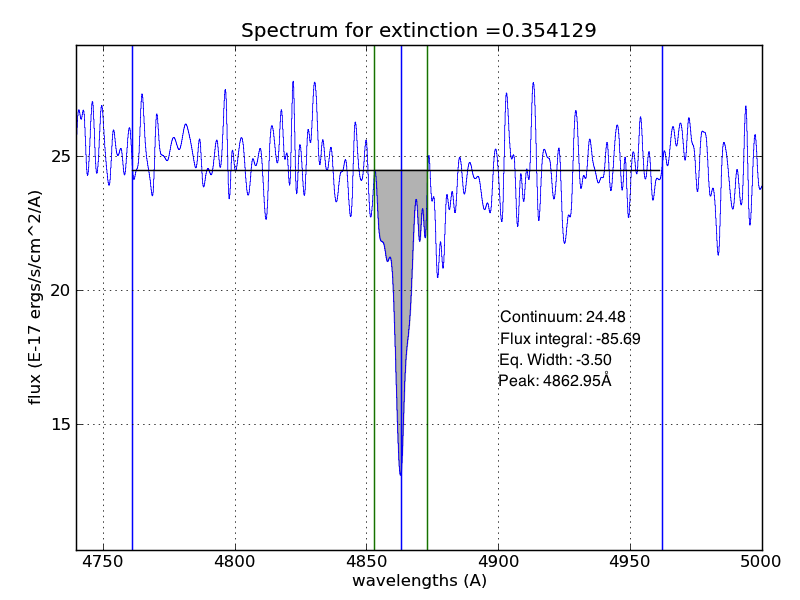
\includegraphics[width=12cm]{../workingexample}\\
Fig. 4. This shows the continuum and equivalent-width estimation. The green lines are each 10$\AA$  away from the central blue line. The blue lines in the extreme left and right are defined at 4761$\AA$ and 4962$\AA$  respectively.
\end{document}